\section{Results}

Figure: \ref{fig:1} shows the difference in radial distance along the y-axis in meters and the number of minutes in that day along the x axis. The small dot along the line y=0 shows the position of the satellite at the specific epoch. The first 6 pass-overs for satellite 21 are shown. It can be seen that each broadcast ephemeris is only within 2m precision for 240 mins (120 mins before and 120 mins after broadcast). After this time, a new ephemeris should be calculated. Figure \ref{fig:2} shows a zoomed in version with the same x and y axis values and units. It clearly represents the large increase in error that occurs after 120 minutes. 
\begin{figure}[h]
	\centering
	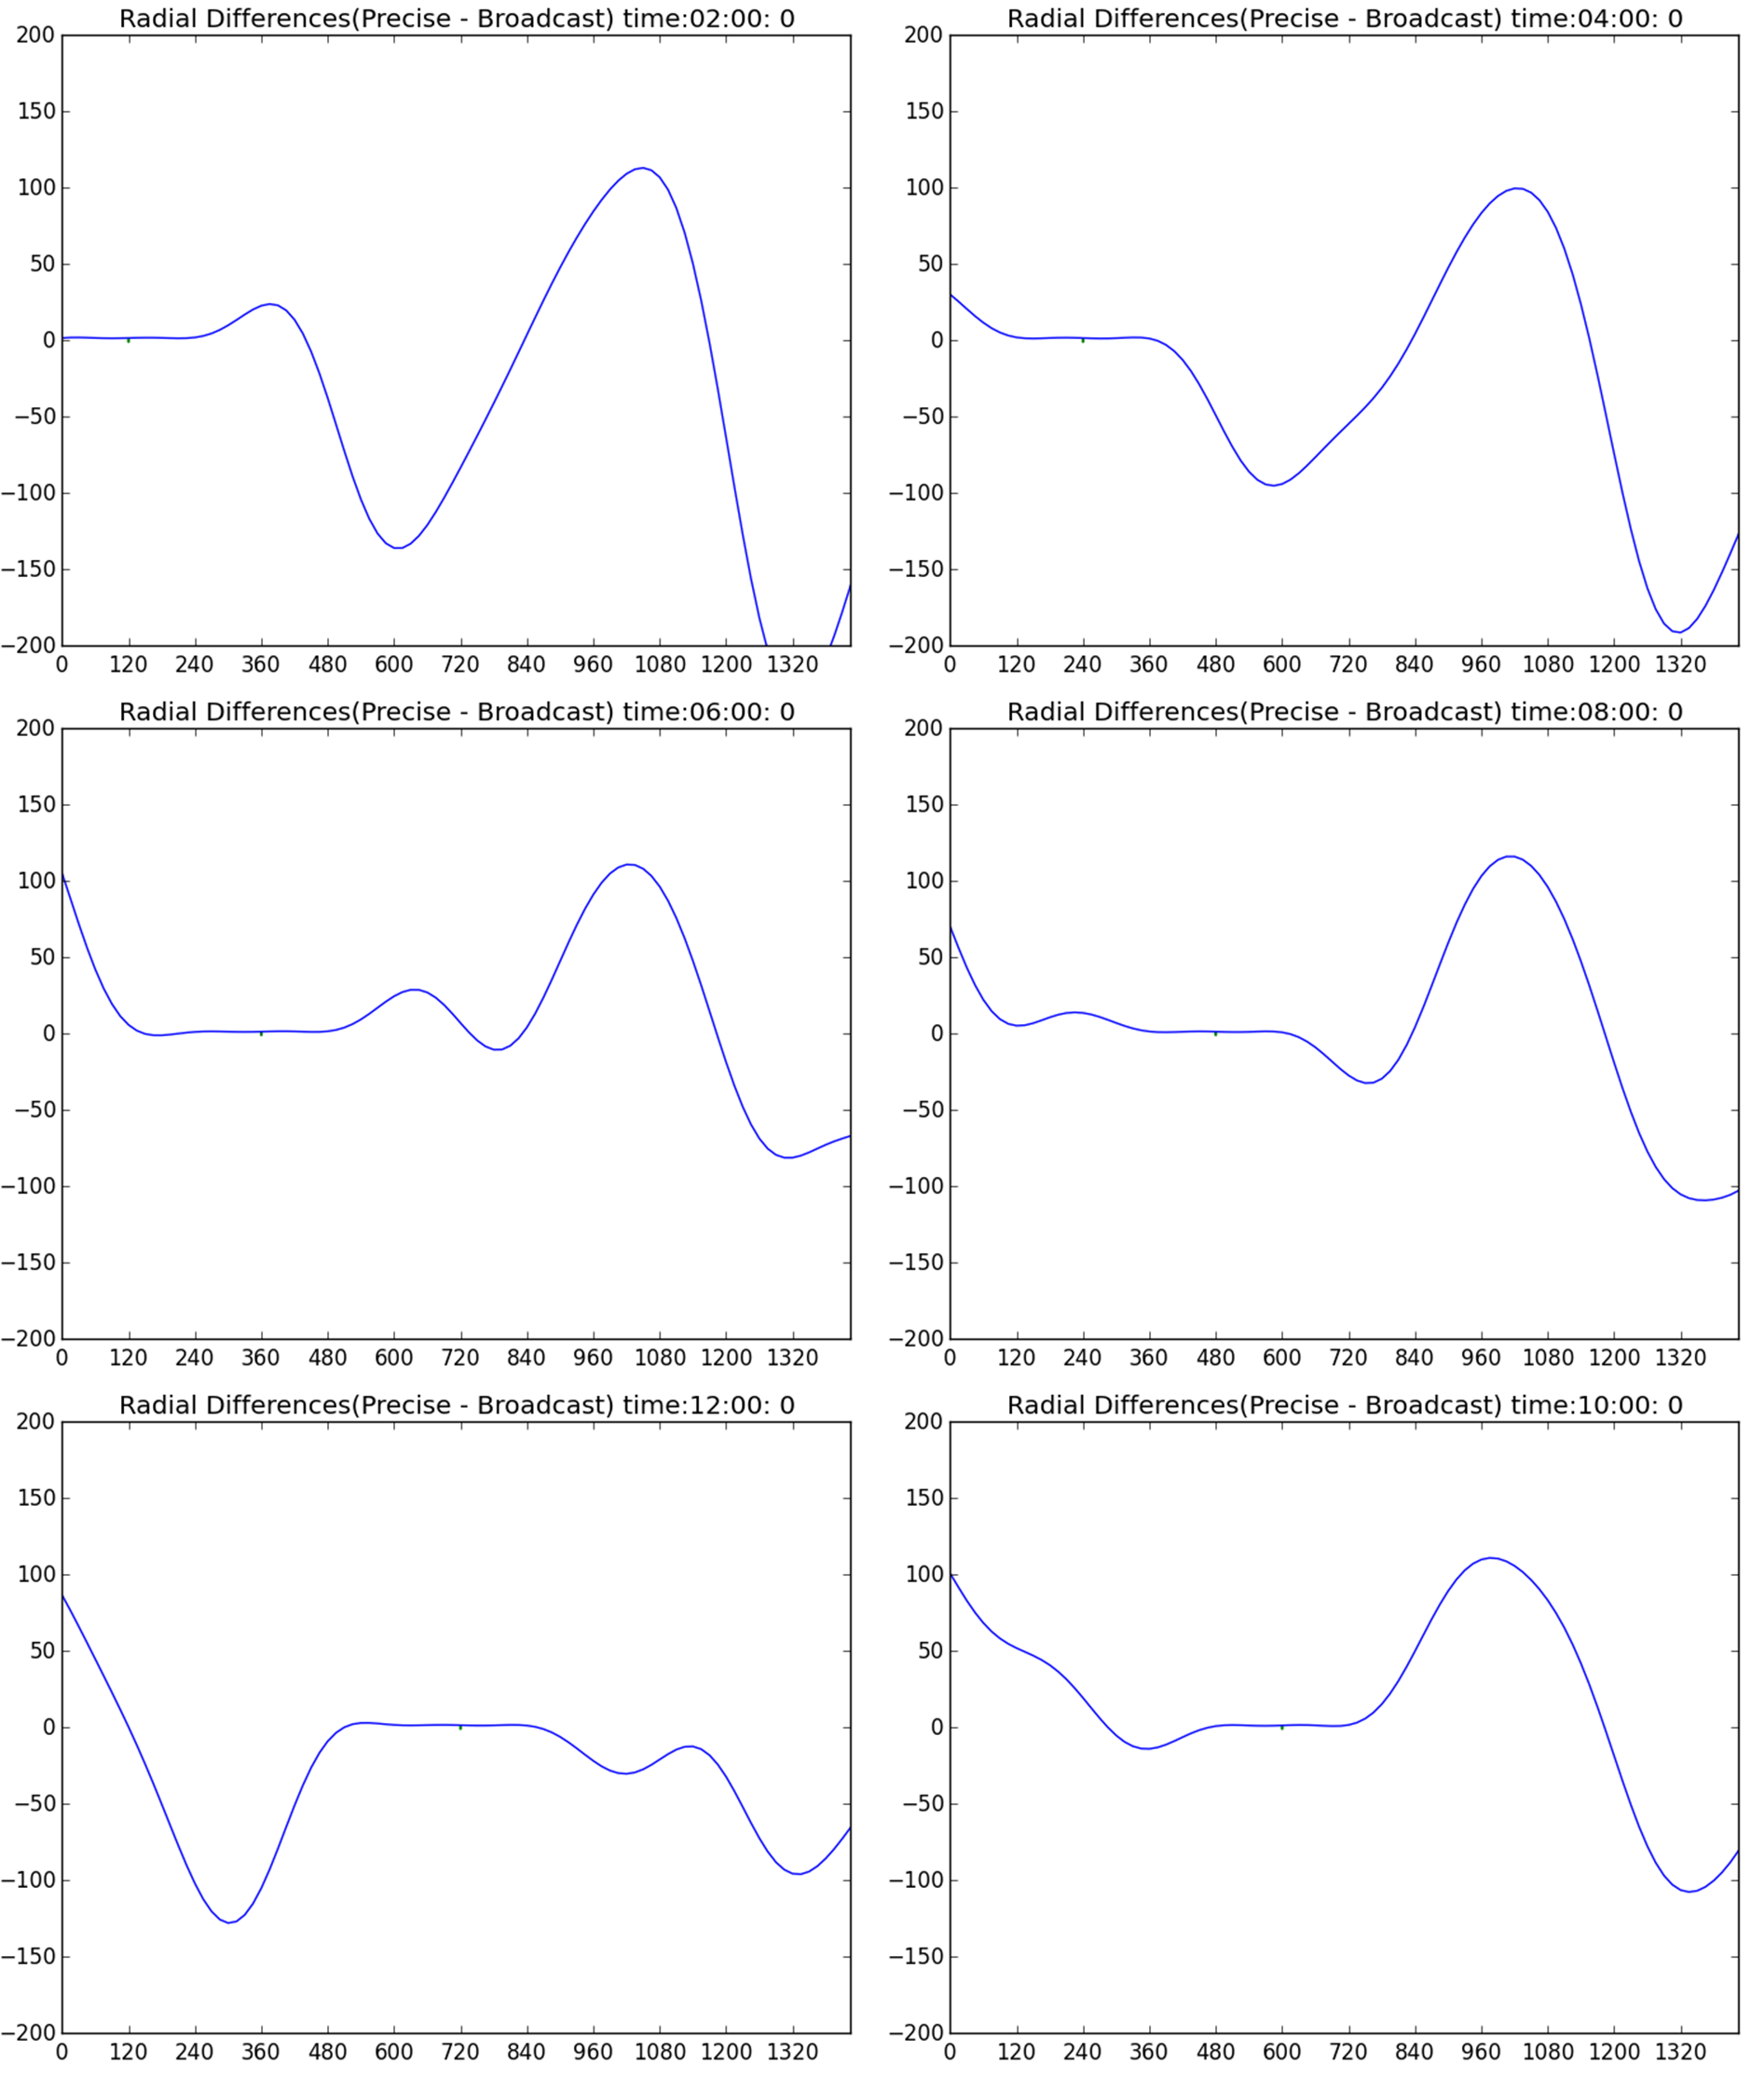
\includegraphics[width=0.6\textwidth]{r1.png}
	\caption{Various Times for Radial Differences}
	\label{fig:1}
\end{figure} 

\begin{figure}[h]
	\centering
	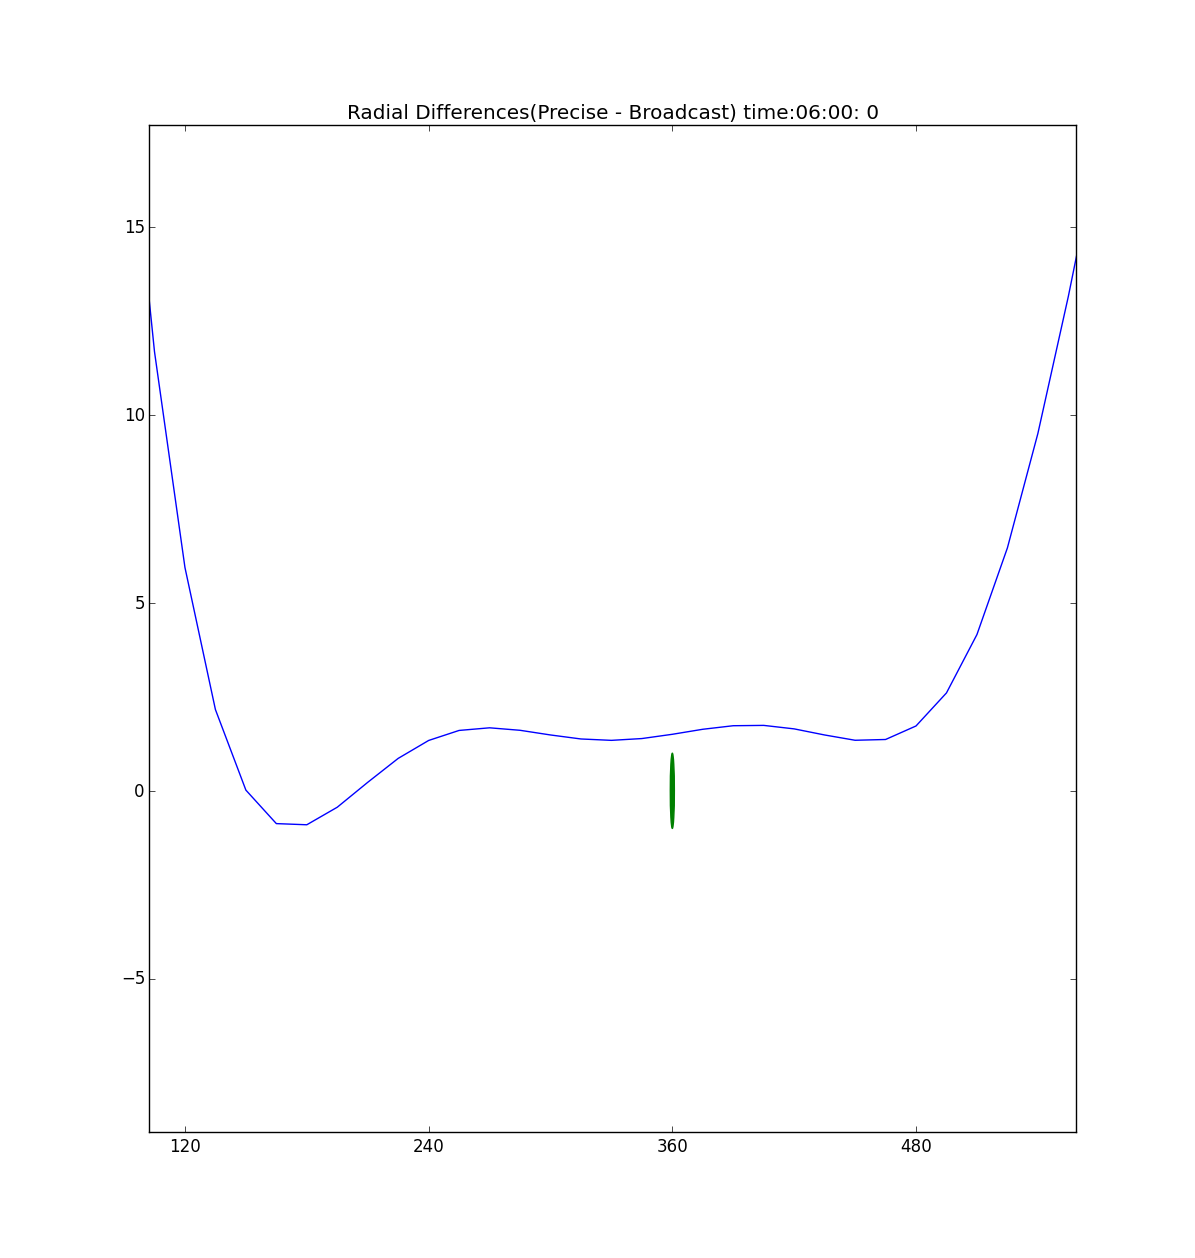
\includegraphics[width=0.6\textwidth]{6.png}
	\caption{Radial Differences (Precise - Broadcast) time-06h00}
	\label{fig:2}
\end{figure} 

% Table generated by Excel2LaTeX from sheet 'Sheet1'
\begin{table}[htbp]
  \centering
  \caption{Radial Differences at 15min Intervals at time t=06h00}
    \begin{tabular}{cccccr}
    \toprule
    88.66267 & 72.17792 & 56.48483 & \textbf{} & \textbf{} & \textbf{} \\
    \midrule
    29.83217 & 19.62730 & 11.69185 & \textbf{} & time  & \multicolumn{1}{c}{RMS (m)} \\
    2.16301 & 0.01845 & -0.87341 & \textbf{} &       &  \\
    -0.43708 & 0.22576 & 0.86294 & \textbf{} & 15mins & 1.41463 \\
    1.60730 & 1.67718 & 1.61113 & \textbf{} & 120mins & 1.49460 \\
    1.38003 & 1.34328 & \textbf{1.39116} & \textbf{} & 180mins & 2.08515 \\
    1.63826 & 1.73277 & 1.74156 & \textbf{} & 240mins & 5.81077 \\
    1.48629 & 1.34558 & 1.36609 & \textbf{} & 300mins & 16.05807 \\
    2.60659 & 4.15989 & 6.46676 & \textbf{} & \textbf{} & \textbf{} \\
    13.16141 & 17.15934 & 21.15208 & \textbf{} & \textbf{} & \textbf{} \\
    27.43905 & 28.91637 & 28.87017 & \textbf{} & \textbf{} & \textbf{} \\
    23.83664 & 19.11163 & 13.38262 & \textbf{} & \textbf{} & \textbf{} \\
    \bottomrule
    \end{tabular}%
  \label{tab:1}%
\end{table}%

\begin{figure}[h]
	\centering
	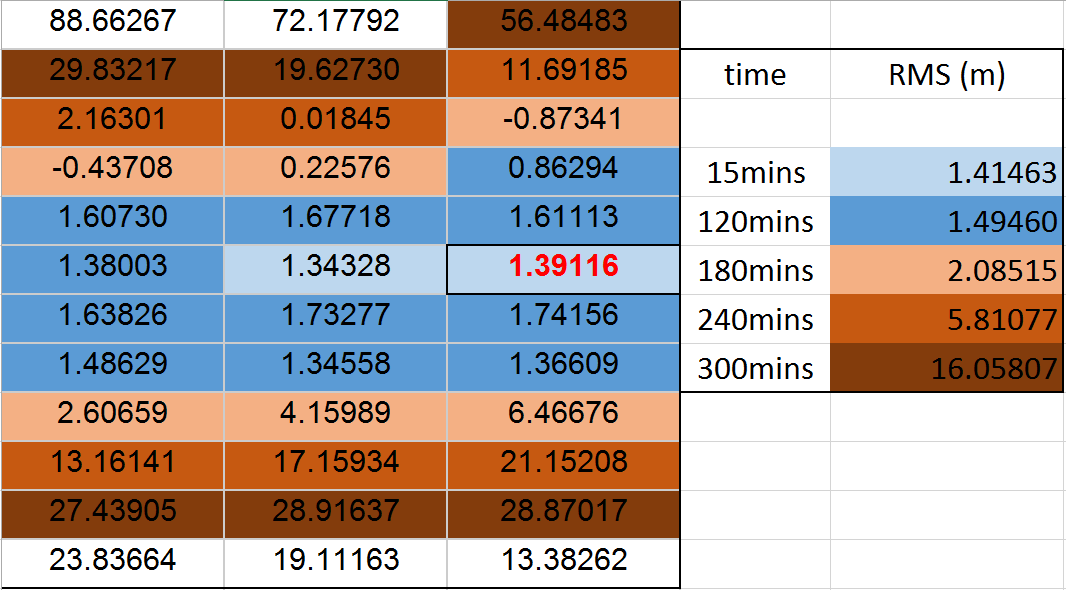
\includegraphics[width=0.8\textwidth]{rms.png}
	\caption{Radial Differences at 15min Intervals (Color Coded)}
	\label{fig:3}
\end{figure} 
The RMS calculations between ephemeris for the epoch 06:00:00 are shown in table \ref{tab:1} and figure \ref{fig:3}. Figure \ref{fig:3} is colour coded for improved visual interpretation.

The mins column show how much time before and after the navigation message. 
 It can be seen that there is not much improvement from 15 mins to 120 mins each side, but RMS rises above 2m after 180 minutes and continues to become unstable reaching over 16m after 5 hours.